\section{Module 10. Upsampling}

\begin{enumerate}
\item Introduction
\newline
Image spatial resolution is limited by several factors. There are for example time of acquisition, organ motions, signal to noise ratio or medical equipment which do not meet the specialized requirements. Specialists usually make relatively small number of 2-D slices. It takes less time but it also results in large slice thickness and spacing between slices. Another example are voxel-wise analysis. The method requires all image volumes of one subject to be analysed in one space. If they are not acquired from the same location (because of the organ motions) the interpolation must be involved.

Interpolation is a method of constructing new points based on the
existing ones. In other words finding a value of a new point in High
Resolution (HR) image based on points in Low Resolution (LR) pictures.

In classical interpolation techniques pixels in LR data $y$ can be
related to the corresponding $x$ values of HR data:
\newline
\centerline {$y_{p}=\frac{1}{N}\sum_{i=1}^{N}x_{i}+n$, where }
\newline
\newline $y_{p}$ is the pixel of LR image at location $p$, \newline $x_{i}$ is each one of the $N$ High Resolution pixels contained within this
LR pixel,
\newline $n$ is some additive noise.

In classical interpolation techniques the High Resolution pixels $x$ are calculated as weighted average of existing LR pixels $y$.
\newline \centerline{$x_{i}=\frac{1}{M}\sum_{i=1}^{M}w_{ij}*y_{j}$, where}
\newline
\newline $w$ are weighted calculated as Euclidean distance between $M$ existing surrounding LR pixels and the coordinates of new ones.   

The biggest problem is that to find High Resolution data from the
Low Resolution values. Unfortunately, there is an infinite number
of values that meet that condition. Interpolation methods can be divided
into three basic techniques.

The first group are the most common ones, like linear or spline-based
interpolation. These techniques assume that it is possible to count
the value of a new point by determination some kind of generic function.
The main disadvantage is that they are correct only for images of
homogeneous regions. As is well known, brain consists of grey substance,
white substance and cerebral spinal fluid, so above-mentioned methods
are not appropriate for MRI images interpolation. The second one is
Super Resolution technique. It is commonly used to increase image
resolution on functional MRI (fMRI) and Diffusion Tensor Imaging (DTI).
The method is based on acquisition of multiple Low Resolution (LR)
images of the same object. It is time consuming and not adequate for
clinical applications.

The last but not least method is non-local patch-based technique which is based on self-similarity of a single image. It is possible to improve resolution by extracting information from a single image instead of acquiring several pictures.

First of all, there is a constraint which says that the original LR image has to be equal to the downsampled version $X$ of the reconstructed image. It is named subsampling consistency constraint which is written as:
\newline \centerline{$y_{p}-\frac{1}{N}\sum{i=1}^{N}X_{i}=0$}
\newline
\newline To make the above equation real, the noise has to be removed. The presence of noise has to be minimalized on the LR image by applying a filter, for example MNLM3D filter for 3D MR images based on Non-Local Means filter. The filter removes the noise effectively without affecting the image structure. 


The aim of this module is to increase MRI image resolution by upsampling.
The input data is a single 320x240 image. After the processing it
is going to be twice as big. To be more specific 640x480 pixels. The
process can be named as double upsampling.

\begin{figure}[H]
\centering{}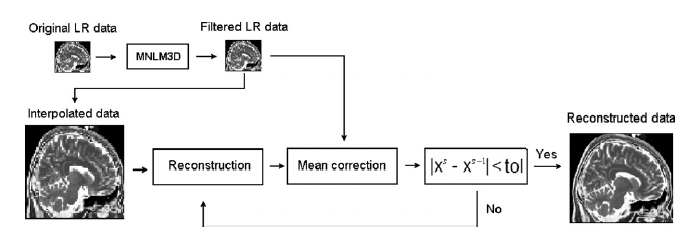
\includegraphics[scale=0.7]{figures/Module_10/Module10_1}\caption{Diagram of the patch-based non-local algorithm \cite{9art1}}. 
\label{fig: Module9_1}
\end{figure}

In a nutshell, the first step of the algorithm is to divide every pixel of LR image into more pixels. Then the patch is designed. It is a rectangle which will be the area of interest. The pixels that are inside the area are taken into account during calculation the values of new points.
After that an appropriate estimator is used to correctly calculate the values of new pixels. Every pixel has to be classified into one of three groups (grey substance, white substance or cerebral spinal fluid).

In order to show how the algorithm is designed the following pictured were generated using exemplary data. At the beginning there is an image 256x256 pixels. 

\begin{figure}[H]
\centering{}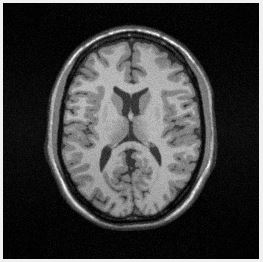
\includegraphics[scale=0.7]{figures/Module_10/Module10_2}\caption{DICOM Low Resolution image 256x256}. 
\label{fig: Module9_2}
\end{figure}

The first step is to add new pixels to increase the resolution M times horizontally and N times vertically. The pixels are equal to zero. After this process an appropriate estimator has to be chosen to make a decision about the values of new points.

\begin{figure}[H]
\centering{}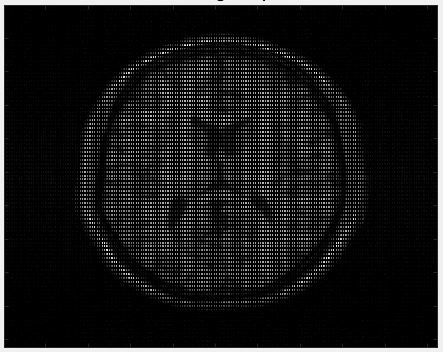
\includegraphics[scale=0.5]{figures/Module_10/Module10_3}\caption{DICOM image with new points with N=2 and M=2}. 
\label{fig: Module9_3}
\end{figure}

Patch-based non-local regularization is used to reconstruct new voxels. The voxel under study is reconstruced using all similar voxels which are placed inside the patch. Contrary to classical techniques which use local neighbourhood of the reconstructed voxel, the proposed method uses the only relevant information, the context of the voxel.

Another step in the algorithm diagram (Fig. \ref{fig: Module9_1}) is mean correction. It has to be applied to ensure that the downsampled reconstructed HR $X$ image is equal to the original $y$ LR one. Thus the local mean value of $X$ fits with the value of the $y$ by adding the corresponding offset.

\centerline{$X=X+NN*(D(X)-y)$, where}


$D$ is an operator that downsamples HR into original LR,
\newline $NN$ is a Nearest Neighbour operator that interpolates LR image to HR.

The Regularization and Correction steps are repeated until no important difference between two consecutive reconstructions. Tolerance is determined by Mean Absolute Difference .

\item Implementation of the method
\newline
The implementation began with making a decision about the input data. The input image has to be 2 dimensional without a noise. The uploaded image will be considered as a 2 dimensional array of double values. Other parameters that will be needed are vertical and horizontal extensions. It has to be a total number. The size of the input array will be multiplied by the number. For example, the image 256x256 pixels with extensions equal to 3 will be 768x768 pixels as an output. The function needs also the window size. In one iteration, the function will take into consideration only pixels witch are inside the window. The loop will stop only when the whole image will be interpolated. To see the results the \textit{plotting} parameter has to be a boolean \textit{True} value. 
\newline The below picture shows the block diagram of the algorithm (Fig. \ref{fig: Module10_4}) with comments added.

\begin{figure}[H]
\centering{}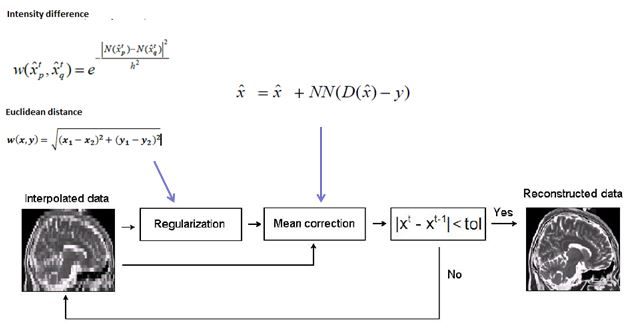
\includegraphics[scale=0.7]{figures/Module_10/Module10_4}\caption{Algorithm block diagram with comments}. 
\label{fig: Module10_4}
\end{figure}

The following steps of the implementation will be discussed:

\begin{itemize}
\item Initial interpolation
\newline To form the input image into the output with chosen size the initial interpolation is needed. As showed in \cite{9art1} the spline interpolation is used. In short, spline interpolation is an interpolation where interpolant is a special kind of piecewise polynomial called spline. It is recommended, because of the fact that the method makes small error even with low degree polynomials for the spline. Taking into consideration the edges the extrapolation was applied. To be more specific, the last row \textit{n} is equal to the previous one \textit{n-1}. The same with the first row, the first column and the last column of the input. To show the results, the extensions are set as 2. The input data is 256x256 pixels. The undermentioned picture (Fig. \ref{fig: Module10_5}) shows the result of the initial interpolation. The scale is included so it is easy to see that the size is twice as big. Now, the zeros (Fig. \ref{fig: Module9_3}) have  nonzero values, so the next steps can be made.


\begin{figure}[H]
\centering{}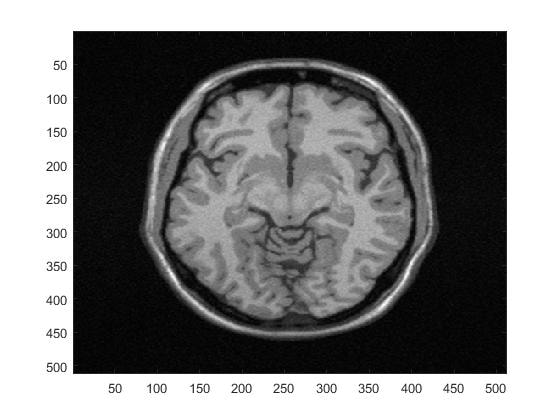
\includegraphics[scale=0.5]{figures/Module_10/Module10_5}\caption{The image after initial interpolation 512x512 pixels}. 
\label{fig: Module10_5}
\end{figure}

\item Regularization
\newline The main functionality is the regularization step. The function makes the square window which contains some pixels. In one iteration of a loop, only the pixels which are inside the window are considered. Next, the window moves and takes another pixels. It is repeated till the end of the image. The main goal is to determine of the weight which will be used at the end.
\newline The first weight is calculated as the difference between the pixels intensities.
\newline 
\centerline {$w_{1}(x, y)= e^{\frac{|N(x)-N(y)|^{2}}{h^{2}}}$, where}
\newline
\newline $N(x)$, $N(y)$ are window and image intensity values,
\newline $h$ is a level, which is equal to the half of the standard deviation of the input image.
\newline The next part of the whole weight is an Euclidean distance weight. It is simply calculated as the Euclidean distance between every pixel in the window and every pixel in the image. It is based on the below equation.
\newline
\centerline{ $w_{2}(x,y)=\frac{\sqrt{(x_{1}-x_{2})^{2}+(y_{1}-y_{2})^{2}}}{h^{2}}$, where }
\newline
\newline $h$ is a level, which is equal to the half of the standard deviation of the input image.
\newline The total weight is calculated as $w_{total}=w_{1}*w_{2}$. The output image is determined as the result of the sum of the multiplication of the weight and the window, divided by the sum of the weight.

\item Mean correction
\newline The mean correction step is a place in the function where the correctness of the equation $X=X+NN*(D(X)-y)$. It was abovementioned, that the downsampled HR has to be equal to the input data.

\item Tolerance checking
At the beginning it was established that only the 2D images will be taken into consideration and the upsampling function will be applied only once, so the step is excluded. There were experiments to upsample the data several times, but the result were not satisfied.

\end{itemize}
\item Results
To visualize the upsampling functionality several output with different parameters are showed (Fig. \ref{fig: Module10_6}, \ref{fig: Module10_7}).

\begin{figure}[H]
\centering{}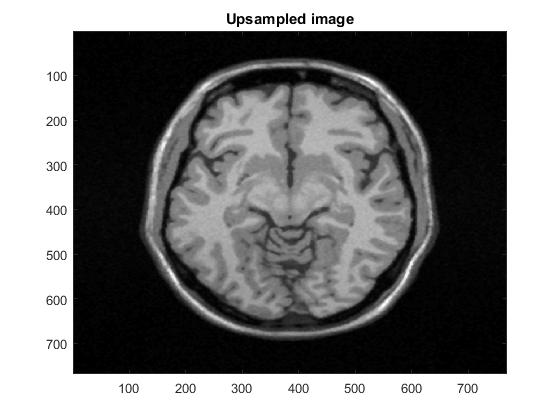
\includegraphics[scale=0.5]{figures/Module_10/Module10_6}\caption{The upsampled image with extensions equal to 3 and window equal to 2}. 
\label{fig: Module10_6}
\end{figure}

\begin{figure}[H]
\centering{}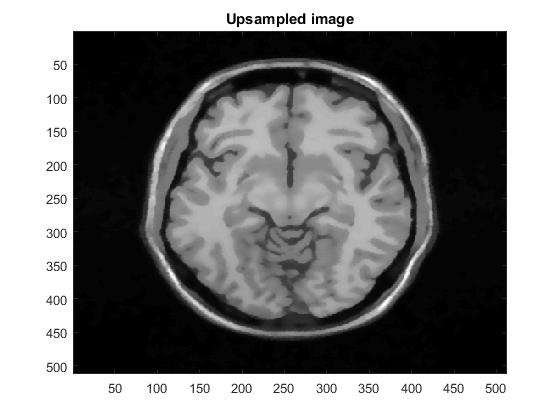
\includegraphics[scale=0.5]{figures/Module_10/Module10_7}\caption{The upsampled image with extensions equal to 2 and window equal to 5}. 
\label{fig: Module10_7}
\end{figure}

To better see the comparison (Fig.\ref{fig: Module10_6_b}, \ref{fig: Module10_7_b})

\begin{figure}[H]
\centering{}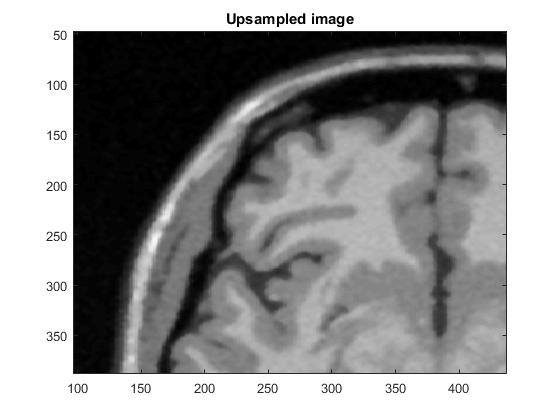
\includegraphics[scale=0.4]{figures/Module_10/Module10_6_b}\caption{The upsampled image with extensions equal to 3 and window equal to 2}. 
\label{fig: Module10_6_b}
\end{figure}

\begin{figure}[H]
\centering{}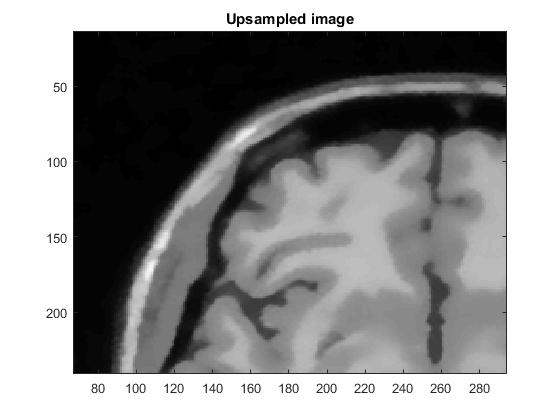
\includegraphics[scale=0.4]{figures/Module_10/Module10_7_b}\caption{The upsampled image with extensions equal to 2 and window equal to 5}. 
\label{fig: Module10_7_b}
\end{figure}

\item Comparison with the other methods
\newline To confirm the better functionality of the proposed method the results will be compared. The other are Linear, Nearest Neighbour, Cubic and Spline interpolation methods (Fig \ref{fig: Module10_l}, \ref{fig: Module10_NN}, \ref{fig: Module10_c}, \ref{fig: Module10_s}). To better see the comparison (Fig. \ref{fig: Module10_thebest}).

\begin{figure}[H]
\centering{}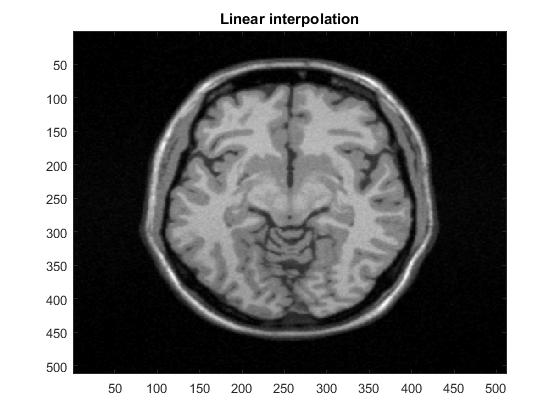
\includegraphics[scale=0.4]{figures/Module_10/Module_10_l}\caption{Linear interpolation}. 
\label{fig: Module10_l}
\end{figure}

\begin{figure}[H]
\centering{}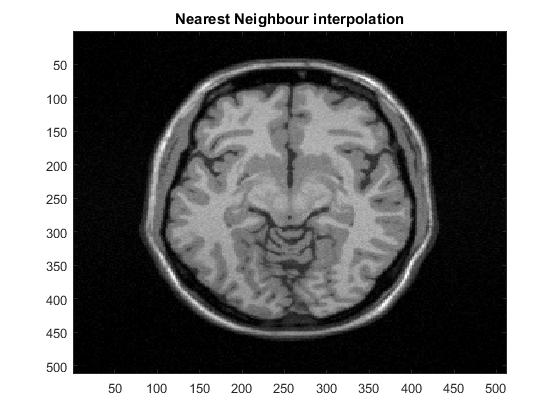
\includegraphics[scale=0.4]{figures/Module_10/Module_10_NN}\caption{Nearest neighbour interpolation}. 
\label{fig: Module10_NN}
\end{figure}

\begin{figure}[H]
\centering{}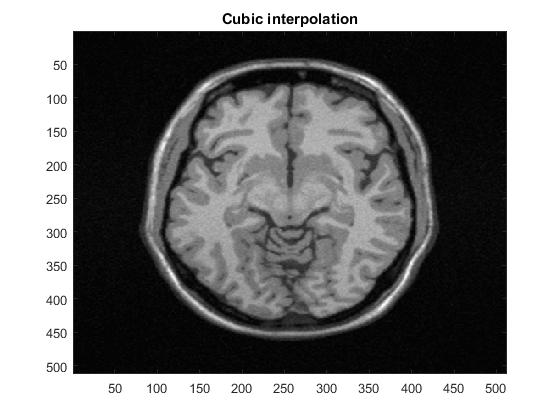
\includegraphics[scale=0.4]{figures/Module_10/Module_10_c}\caption{Cubic interpolation}. 
\label{fig: Module10_c}
\end{figure}

\begin{figure}[H]
\centering{}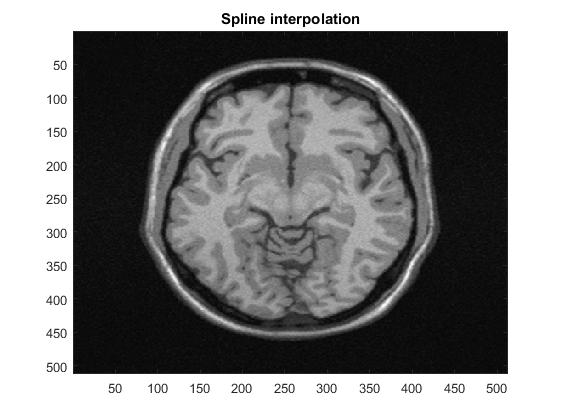
\includegraphics[scale=0.4]{figures/Module_10/Module_10_s}\caption{Spline interpolation}. 
\label{fig: Module10_s}
\end{figure}

\begin{figure}[H]
\centering{}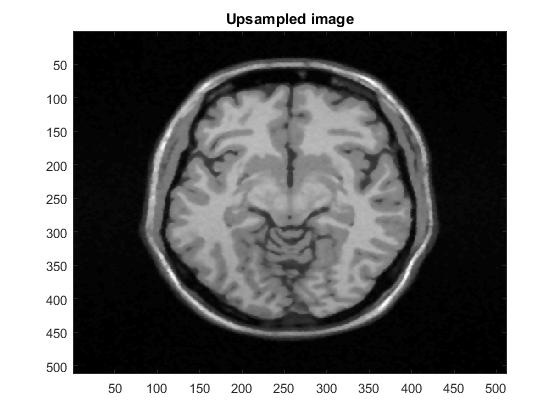
\includegraphics[scale=0.4]{figures/Module_10/Module_10_thebest}\caption{Proposed method}. 
\label{fig: Module10_thebest}
\end{figure}

\item Conclusions
\newline In conclusion, implementation of a new interpolation method met with success. Unquestionably, the proposed method gives better results than other popular interpolation methods.
\end{enumerate}

\hfill{}\\
\textbf{List of References}\\
\cite{9art1}
\cite{9art2}